\documentclass[a4paper,12pt,abstracton]{scrartcl}
\usepackage[ngerman, english]{babel}
\usepackage[utf8]{inputenc}
\usepackage[T1]{fontenc}
\usepackage{graphicx}
\usepackage{lipsum}
\usepackage{blindtext}
\usepackage{color}
\usepackage{setspace}
\usepackage{hyperref}
\usepackage[printonlyused]{acronym}
\usepackage{amsmath}
\usepackage{amsfonts}
\usepackage{amssymb}
\usepackage[export]{adjustbox}
\usepackage{subcaption}
\usepackage{makecell}
\usepackage[]{units}
\usepackage{natbib}
\usepackage{aas_macros}
\usepackage{enumerate}


\title{Bachelorarbeit}
\author{Sophia Milanov}
\date{\today}

\begin{document}
\bibliographystyle{glenn} 
\pagenumbering{roman}

\onehalfspacing
\begin{titlepage}
\begin{center}
 
\Large\textbf{Department of Physics and Astronomy\\
University of Heidelberg}

\vspace{15cm}

\normalsize
Bachelor Thesis in Physics\\
submitted by \\
\vspace{0.5cm}
\Large\textbf{Sophia Milanov}\\
\normalsize
\vspace{0.5cm}
born in Düsseldorf (Germany)\\
\vspace{0.5cm}
\Large\textbf{2016}
\normalsize
\newpage
\mbox{}
\thispagestyle{empty}
\newpage
\
\Large\textbf{Hunting for Intermediate-Mass Black Holes in simulated Globular Clusters using Integrals of Motions}

\vspace{18cm}

\normalsize
This Bachelor Thesis has been carried out by Sophia Milanov at the\\
Max Planck Institute for Astronomy in Heidelberg\\
under the supervision of\\
Dr. Glenn van de Ven

\vfill
\end{center}

\end{titlepage}


\begin{abstract}
\hspace{-12pt}In this thesis we carried out investigations in action space of simulated \acp*{GC} to examine if the method of integrals of motion is useful to find signatures of \acp*{IMBH}, whose detection is still highly controversial. We investigated four simulated \acsp*{GC}, two of which contain an \acs*{IMBH}. In position-momentum space we showed that the \ac{IMBH} leads to a central cusp in the stellar density distribution and to an increased velocity dispersion around the \ac{IMBH} - both well-known characteristics of \acp{IMBH} in simulated \acp{GC}. To study the \ac{GC} stars in action space, we implemented an object-oriented analysis code to a) calculate the gravitational potential from the stellar density, b) determine the pericentre, apocentre and guiding-star radius of the stars of the GC orbits and c) evaluate the actions and classical integrals of motions (i.e., energy and angular momentum) from the current positions and velocities of the stars. We found signatures of the \acsp*{IMBH} in distributions of the radial action versus the energy, the angular momentum and the guiding-star radius. In particular, we found stars on circular orbits very close the the central \ac{IMBH}. These kind of orbits do not seem to be populated in \acp{GC} without \ac{IMBH}. We tested these signatures using a wrong potential to calculate the integral of motions and showed that they are robust signatures of a presence of \acsp*{IMBH}. 
%\vspace{2cm}
\begin{center}
 \textbf{Zusammenfassung}
\end{center}
In dieser Arbeit untersuchten wir simulierte Kugelsternhaufen im Wirkungs-Winkel Raum durch, um zu testen, ob diese Methode nützlich ist, Charakteristika von mittelschweren schwarzen Löchern zu finden, deren Entdeckung höchst umstritten ist. Wir untersuchten vier simulierte Kugelsternhaufen, von denen zwei ein mittelschweres schwarzes Loch enthalten. Nach der Analyse im Phasenraum wechseln wir in den Wirkungs-Raum mit Hilfe der von Dichteprofilen abgeleiteten Potentiale. Um die Kugelsternhaufen im Wirkungs-Raum zu untersuchen, implementierten wir einen Objekt-orientierten Code, der a) das Gravitationspotential der Sternedichte, b) Perihel, Aphel und Leitstern-Radius der Sterne in den Kugelsternhaufen und c) die Wirkungen und die klassischen Bewegungsintegrale (Energie und Drehimpuls) mit Hilfe der aktuellen Position und Geschwindigkeit berechnete. Wir fanden Charakteristika des mittelschweren schwarzen Lochs, genauer gesagt Sterne auf Kreisbahnen sehr nah am mittelschweren schwarzen Loch, die bei den Kugelsternhaufen ohne schwarzes Loch nicht auftreten. Wir testen diese Signaturen mit einem falschen Potenzial, aus dem wir die Bewegungsintegrale berechnen und zeigen, dass diese Signaturen eines schwarzen Loches robust sind.
\end{abstract}

\newpage
\addtocontents{toc}{}
\tableofcontents

\newpage
\pagenumbering{arabic}



\section{Introduction}

\subsection{Motivation}
In this thesis we will apply integrals of motion as actions to  \ac{GC}s to investigate possible signatures of \ac{IMBH}s. 
\subsection{What is a globular cluster in the Milky Way?}\label{sec1.2}
\ac{GC}s are self-gravitating, gas-free systems of 10\(^6\) to 10\(^8\) stars which are spherically grouped. There are about 150 of them in the \ac{MW}. As some of the oldest stellar populations in the universe we can obtain much information about the evolution of the \ac{MW}. Formerly seen as very simple system with only one stellar population and without rotation recent research revealed a much higher complexity of these systems. \color{red} nachlesen, wie das genau mit stellar populations und rotation und models ist \color{black}
\\In this \ac{CMD} the visual magnitude is plotted against the B-V color. It's color coded by the mass of the star. A star's position can be interpreted as its evolution stage. Most of the stars are set in the main sequence. They fusion hydrogen in their cores. There are two main sequence lines one upon the other. These occur due to binary systems. These binary systems represent about \color{red} percentage \color{black} \% of the stars in the \ac{GC}. The main sequence turn-off is depending on the age of the system and is used as indicator for such. Beyond this turn off point there are so called blue stragglers which are remnants of stellar collisions (B\&T p.628). Continuing from the turn off point there is the red giant branch consisting of stars still fusing hydrogen but only in a shell surrounding a degenerate helium core. They are inflated with a radius much higher than the main sequence stars but have only a very low temperature. At the end of the red giant branch lies the horizontal branch. Its stars have sun-like masses and burn helium in their core and hydrogen in a surrounding shell. In the lower left corner white dwarfs are located. They are stellar remnants which have burnt all of their resources. \color{red} nochmal über \ac{CMD} durchlesen und alle branches erwähnen \color{black} In 3.1. we will compare the \ac{CMD} to isochrones which describe the actual distribution of stars in the different stages for a given age and metallicity. 
\\In their centre \ac{GC}s could contain an \ac{IMBH}. These could be the missing link between stellar mass black holes and \ac{SMBH} as origin of the \ac{SMBH}. Currently there are two different kinematic methods trying to detect \ac{IMBH}s. As an example there are the unresolved/integrated IFU kinematics which result in a signature of an \ac{IMBH} for NGC 6388 and resolved/discrete kinematics which don't yield \ac{IMBH}s. \color{red} include graph of paolo's talk? \color{black} To get more certain methods we test if we can derive a signature of the \ac{IMBH} by computing and comparing actions of the stars.


%\includegraphics[width=\textwidth]{Plots/color_magnitude_diagram}
\subsection{Actions \& orbits}
Orbits contain all information about the potential of a system in their position and velocity coordinates following Newtons 2nd law. From the orbit distribution function we can draw inferences about the history of the system. Since there are many possible orbits but the stars are only on some of them questions are raised. How do they come on these special orbits? What do these orbits tell us about the evolution of the system? 
\\There are some examples when orbits enabled discoveries or confirmed them: 
\begin{itemize}
\item Seen from the earth Mars' position moves over the sky as a loop. That implies that the earth is not the centre of the universe!
\item Neptune/Uranus \color{red} noch mal nachlesen \color{black}
\item From rotation curves of galaxies we see that stars move faster than expected by mass of luminous matter. There has to be more matter interacting via gravitational forces. This has led to the theory of dark matter.
\item Mercury's orbit differs hugely from calculated Kepler orbit. This is because of its migrating pericentre. Due to the proximity to the sun gravitational forces are so strong that we need to apply general relativity.
\item The \ac{SMBH} Sagittarius A*  was detected by observations of the orbits around the black hole and resulting mass calculations.
\end{itemize}
Some examples for orbit distribution functions are the asteroid belt, the distribution function of moons around planets which allows feedback connections to formation and bonding of different planet types and spiral galaxies where stars of different parts(thin disc, thick disc, bulge, halo) have different orbits (dynamical distinct) and different metallicity (chemical distinct).
\\\\
Actions are integrals of motion and are the distinct description of orbits. They are constant with time. Known for a long time they are extremly difficult to calculate. Actions of our solar system can be calculated easier since we know the potential. With nowadays supercomputers it's finally possible to compute actions of more complex and less explored systems.





\newpage
\section{Method \& Theory}\label{method_theory}
\subsection{Stellar population in GC}\label{cmd_theory}
The typical stellar components of a \ac{GC} can be seen in a \ac{CMD}. Figure \ref{fig:cmd} shows the \ac{CMD} of a simulated \ac{GC} where the visual magnitude is plotted against the B-V color. It's color coded by the mass of the star. 
\begin{figure}[htbp]
\centering
	\includegraphics[width=0.5\textwidth]{Plots/color_magnitude_diagram.png}
	\caption{Color magnitude diagram of SIM 1.}
	\label{fig:cmd}
\end{figure}
A star's position can be interpreted as its evolution stage. Most of the stars are set in the main sequence. They fusion hydrogen in their cores. There are two main sequence lines one upon the other. These occur due to binary systems whose flux is given by the sum of the single fluxes of the single components, and therefore appear redder and more luminous. These binary systems represent about \unit[5]{\%} of the stars in the \ac{GC}. The position of the main sequence turn-off depends on the age of the system and therefore can be used as an indicator to determine the cluster's age. Isochrones are curves of evolutionary stages of stars of a \ac{SSP} having the same age and metallicity but different masses. Bluewards of this turn off point following the trend of main sequence stars, there are so called "blue stragglers" which are remnants of stellar collisions or interacting binaries \citep[p.628]{2008gady.book.....B}. Continuing from the turn off point there is the red giant branch consisting of stars still fusing hydrogen but only in a shell surrounding a degenerate helium core. They are inflated with a radius much higher than the main sequence stars but have a much lower surface temperature. These are the brightest stars of a \ac{GC}. On the upper part of the red giant branch lies the horizontal branch. Its stars burn helium in their core and hydrogen in a surrounding shell. In the lower left corner white dwarfs are located. They are stellar remnants which have burnt all of their resources. In a typical \ac{GC} dark stellar remnants like stellar black holes and neutron stars are present but not visualised in the \ac{CMD}. 
\subsection{Kinematic profiles of globular clusters}\label{kin_prof_theory}
We will investigate \acp{GC} in phase space by analysing the stellar kinematic profiles (such as velocity dispersion and anisotropy profiles) and the spatial distribution of stars (density profiles and potential). 
\par The stellar velocity dispersion quantifies the spread of different velocities stars at given positions can have. It is defined as the standard deviation of the velocity distribution  
\begin{equation}\label{eq:vel_disp}
\sigma_\mathrm{i}(\mathrm{r})\equiv\sqrt{\left\langle(\mathrm{v_i}(\mathrm{r})-\langle \mathrm{v_i}(\mathrm{r})\rangle)^2\right\rangle}=\sqrt{\left\langle \mathrm{v_i}(\mathrm{r})^2\right\rangle-\langle \mathrm{v_i}(\mathrm{r})\rangle^2} \qquad\qquad \mathrm{i=r,\theta,\phi}.
\end{equation} Here v describes the actual velocity of the star while \(\left\langle \mathrm{v}\right\rangle\) specifies the mean of the velocities of all considered stars. For a spherical system it is best to calculate them in spherical coordinates \(\mathrm{r},\theta,\phi\) respectively \(\mathrm{v_r,v_{\theta},v_{\phi}}\). If the \ac{GC} contains an \ac{IMBH} the velocity dispersion towards the centre is expected to increase. 
\par To quantify the anisotropy of the system we use the anisotropy parameter \(\beta\) 
\begin{equation}\label{eq:anisotropy}
\mathrm{\beta(r)\equiv1-\frac{\sigma_\theta ^2(r)+\sigma_\phi ^2(r)}{2\sigma_r ^2(r)}}
\end{equation} taken from \citep[eq. 4.61]{2008gady.book.....B}. If \(\beta\) is positive the anisotropy is radial, if it is negative the anisotropy is tangential and if \(\beta\approx0\) then the system is isotropic.
\subsection{Density \& potential}\label{dens_pot_theory}
\subsubsection{Density of a collisionless stellar system}
\begin{equation}\label{eq:density}
\rho(\mathrm{r})=\frac{\sum_{\mathrm{r=r_{in}}}^{\mathrm{r_{out}}}\mathrm{M(r)}}{\mathrm{V(r_{out}-r_{in})}}
\end{equation}

\subsubsection{Generating the potential from Poisson's equation}
Since the system is spherically potential and force only depend on the distance from the centre r. The potential \(\Phi\) can be derived from the Poisson's equation \begin{equation}\label{eq:Poisson}
\mathrm{\Delta\Phi(r)=4\pi G \rho(r)}
\end{equation}
with the gravitational constant G = \unitfrac[\(6.674\cdot10^{-11}\)]{\(\mathrm{m}^3\)}{\(\mathrm{kg\ s}^2\)} \citep{2015arXiv150707956M} and the density \(\rho\) depending only on the distance as well. Due to the spherical symmetry the potential can be calculated by 
\begin{equation}
\mathrm{\Phi(r)=-\frac{G}{r}\int_0^r{\mathrm{d}M(r')}-G\int_r^{\infty}{\frac{\mathrm{d}M(r')}{r'}}=-4\pi G\left[\frac{1}{r}\int_0^r\mathrm{d}r'r'^2\rho(r')+\int_r^{\infty}\mathrm{d}r'r'\rho(r')\right]}
\end{equation} with dM describing the mass of spherical shells as proved by \citet[eq. 2.28]{2008gady.book.....B}. 
\subsubsection{Other potential models}
Kepler potential IMBH\\Plummer model\\short: isochrones
\subsection{Orbits \& integrals of motion}\label{orbit_int_of_motion_theory}
\subsubsection{Classical integrals of motion in spherical potential}
\color{red} how does the orbit in a spherical potential look \color{black}
In a dynamical system the mass distribution is described by the form of theoretically existent orbits (\(\vec{x}(t),\vec{v}(t))\). Position and velocity are linked with six coordinates and contain all information about the potential. With Newton's 2nd law we get the connection between potential \(\Phi(\vec{r})\)and acceleration \(\vec{a}\) which is \[\vec{F}(\vec{r})=-\nabla\Phi(\vec{r})=m\cdot\vec{a}.\]  We calculate the density by binning the masses on logarithmic equally distributed shells \color{red} write density formula? \color{black} and solve the integrals of the Poisson's equation numerically by using the Gauss-Legendre quadrature \[\int_a^b f(x)dx = \frac{b-a}{2}\sum_{i=1}^n w_i f\left(\frac{b-a}{2}x_i+\frac{a+b}{2}\right)\] where the points \(x_i\) and the weights \(w_i\) are derived from the Legendre polynomials.\\ Since the orbit is described by position and velocity at each time step we use the numerical leapfrog method which is a second-order time reversible integrator. \(X_i\) and \(v_i\) are calculated by 
\begin{align*}
x_{i+1}=x_i+v_i\Delta t+\frac{a_i(x_i)}{2}\Delta t^2 \\
v_{i+1}=v_i+\frac{a(x_{i+1})+a(x_i)}{2}\Delta t.
\end{align*}

\color{red} gcs are collisional clusters but we assume them as collisionless \\ time evolution of actions \color{black}
\subsubsection{The effective potential}
\begin{figure}[htbp]
\centering
	\begin{subfigure}{0.475\textwidth}
	\includegraphics[width=\textwidth]{Plots/eff_potential_bartelmann.png}
	\caption{General potential of a central field. The black line is the potential which is the difference between the effective potential (yellow line) and the centrifugal potential (red line). If the effective potential is positive the object is unbound while having a negative potential the object moves on a bound orbit. The points where the effective potential equals the total energy are the peri- and apocentre (r\(_1\) and r\(_2\)) of the orbit. The point with the lowest effective potential is the guiding star radius. This is the distance a star with given angular momentum would have on a circular orbit. [Bartelmann Skript Theo 1]}
	\label{fig:eff_potential_bartelmann}
	\end{subfigure}
	\hfill
	\begin{subfigure}{0.475\textwidth}
	\includegraphics[width=\textwidth]{Plots/pot_eff_theory_part.pdf}
	\caption{Effective potential of a random star of SIM 1 (blue line). The total energy of the star (red line) is -1.88e-24 \(\mathrm{pc}^2/\mathrm{s}^2\). The intersections of energy and effective potential are the peri- and the apocentre of the star (magenta and black lines) and the minimum of the effective potential (green line) is the guiding star radius.}
	\label{pot_eff_theory_part}
	\end{subfigure}
\caption{Effective potentials.}
\label{fig:pot_eff_theory}
\end{figure}
\subsubsection{Actions}
Stars in spherical symmetric potential are fully described by their actions \begin{equation}
J_i=\frac{1}{2\pi}\oint_{\gamma_i}\vec{p}\cdot d\vec{q} \qquad\qquad i=r,\theta,\phi
\end{equation} which are used as coordinates in action space
These actions are integrals of motion. For most potentials actions can't be described analytically. The actions of a spherical system are derived from angular momentum, energy and potential. Only the potential is depending in r. Energy and angular momentum as well as resulting actions are constant over time and orbit. The azimuthal action J\(_\phi\) and the latitudinal action J\(_\theta\) can be evaluated simply. To calculate the radial action J\(_r\) we have to solve an integral numerically. Actions of a spherical potential are found to be \begin{align}
J_\phi=L_z, \\ J_\theta=L-|L_z|, \\ J_r=\frac{1}{\pi} \int_{r_{min}}^{r_{max}} \mathrm{d}r \sqrt{2E-2\Phi(r)-\frac{L^2}{r^2}}.
\end{align}\color{red} Should I write down the derivation of the actions (B\&T p.220) or just the results (B\&T p.221, 3.221,3.223,3.224)?\color{black} \\ The pericenter \(r_{min}\) and the apocenter \(r_{max}\) as well as the guiding star radius \(r_g\) can be found in the effective potential \begin{equation}
V_L(r)=V(r)+\frac{L^2}{2mr^2}.\  \color{red} \mathrm{m\ should\ be\ left\ out\ right?} \color{black}
\end{equation} \color{red} Bartelman Theo 1 Skript p59 formula 6.27. \\ \color{black} In the peri- and apocenter the effective potential equals the total energy since the stars do not have any kinetic energy there. That results in following function which is to solve: \[\left(\frac{1}{r}\right)^2+\frac{2\cdot (\Phi-E)}{L^2}=0.\] \\ The guiding star radius is the distance at which a star with given total angular momentum would have a circular orbit. This is at the minimum of the effective potential. To get \(r_g\) we have to solve \[r\sqrt{r\frac{\partial\Phi}{\partial r}}-|L|=0\] where \(\sqrt{r\frac{\partial\Phi}{\partial r}}=v_{circ}\) is the circular velocity. This distance is used to have a better comparison of the actions since in the snapshot the stars are at a random position on their orbit.
\subsubsection{Numerical orbit integration}
\subsection{Examples for orbits in spherical potentials}

\newpage
\section{Analysis}

\subsection{Description of the simulation}
We consider a set of Monte Carlo cluster simulations, developed with the Monte Carlo
code MOCCA of Hypki et al. 2013 (see also Giersz et al. 1998). The simulations
include an initial mass function, stellar evolution, primordial binaries, and a
relatively high number of particles, providing a realistic description of the
long-term evolution of \acp{GC} with a single stellar population.

All the simulation had a metallicity of [Fe/H]=$-$1.3 and a Kroupa (2001) initial
mass function. The first simulation (from Giersz et al. 2015, kindly shared by the
authors) contain an \ac{IMBH} of $10^4$ M$_\odot$ and its initial condition is drawn from a
King model with concentration parameter W$_0 $=6, 6.9$\cdot10^5$ initial number of particles,
95\% of which are binary systems. We consider two snapshots of the simulation on at
10 and one at 7 Gyr. We call these snapshots SIM1-IMBH and SIM2-IMBH, respectively.
Other two simulations (from Downing et al. 2010, kindly shared by the authors), do
not contain an \ac{IMBH} and have an initial number of particles of 5$\cdot10^5$ and 2$\cdot10^6$, 10\%
of initial binaries, and initial conditions drawn from a Plummer (1911) model with a
ratio between the initial tidal radius and half-mass radius of 75. We consider a 11
Gyr snapshot for both simulations and we call them SIM3-NOIMBH and SIM4-NOIMBH,
respectively.

We summarize in Table \ref{tab:overview_simulation} the properties of the simulations for the time-snapshots
considered. 


\begin{table}[htbp]
\centering
\begin{tabular}{ c | c | c | c | c | c }
\makecell{Name of the \\simulation} & \makecell{Number of \\ particles} & Total mass [M\(_\odot\)]& \makecell{Mass of the \\ \ac{IMBH} [M\(_\odot\)]}& r\(_\mathrm{m}\) [pc] & Age [Gyr]\\
\hline			
  SIM 1 - IMBH & 1026735 & 3.09\(\cdot 10^5\) & 10102 & 4.13 & 10\\
  SIM 2 - IMBH & 1079376& 3.26\(\cdot 10^5\) & 8902.3 & 3.58 & 7\\
  SIM 3 - NOIMBH & 468627& 1.73\(\cdot 10^5\)& 0 & 7.89 & 11\\
  SIM 4 - NOIMBH & 1851556& 6.70\(\cdot 10^5\)& 0 & 5.41 & 11\\

\end{tabular}
\caption{Overview of the data of the simulations. We show the basic properties of each simulation which are numper of particles, the total mass, the mass of the \ac{IMBH}, the half mass radius and the age. The half mass radius is defined by the radius which includes half of the mass of the whole system.}
\label{tab:overview_simulation}
\end{table}

The output of the simulations relevant for our work are for each star: the position
vector x, the velocity vector v in Cartesian and polar coordinates, mass, luminosity, magnitude b and v band and whether
the star is a binary or not.
\\
To get familiar with the simulation we first have a look at the distribution of the star positions.
\begin{figure}[htbp] 
\centering
\begin{subfigure}{0.9\textwidth}
	\centering
  	\includegraphics[width=\textwidth]{Plots/position_scatter_plot_IMBH.pdf}
  	\caption{SIM 1 \& SIM 2. The \acp{GC} are spread until 100 pc with most of the stars located in the inner 40 pc.}
 	\label{fig:pos_scat_IMBH}
\end{subfigure}
\\
\begin{subfigure}{0.9\textwidth}
	\centering
  	\includegraphics[width=\textwidth]{Plots/position_scatter_plot_noIMBH.pdf}
  	\caption{SIM 3 \& SIM 4. The \ac{GC} is spread until 90 pc (SIM3) and until 60 pc (SIM4).}
 	\label{fig:pos_scat_noIMBH}
\end{subfigure}

\caption{Spatial distribution of stars in the simulated \acp{GC}. The stars are distributed spherically with most of the stars in the inner part. The stars of the \acp{GC} with \ac{IMBH} are less spread in the outer parts except very few which are far outside. This is simply due to the different initial concentration conditions of the simulations. In the \acp{GC} without \ac{IMBH} the stars in the outer part are less accumulated but the furthermost stars still in the main sphere.}
\label{fig:position_scatter}
\end{figure}

\begin{figure}[htbp] 
\centering
	\begin{subfigure}{0.9\textwidth}
		\centering
	  	\includegraphics[width=\textwidth]{Plots/velocity_scatter_IMBH.pdf}
	  	\caption{SIM 1 \& SIM 2. The stars' velocities are spread until 120 km/s with most of them reaching 30 km/s.}
	 	\label{fig:vel_scat_IMBH}
	\end{subfigure}
	\\
	\begin{subfigure}{0.9\textwidth}
		\centering
	  	\includegraphics[width=\textwidth]{Plots/velocity_scatter_noIMBH.pdf}
	  	\caption{SIM 3 \& SIM 4. The stars' velocities are spread until 15 km/s for SIM 3 whereas they spread until 40 km/s for SIM 4.}
	 	\label{fig:vel_scat_noIMBH}
	\end{subfigure}

\caption{Velocity distribution of stars in the simulated \acp{GC}. The velocities are isotropically spread around \(\vec{v}=0\). Most of the stars have low or no velocity while a few have high velocities in different directions. There are no overall streaming motions.}
\label{fig:velocity_scatter}
\end{figure}


\subsection{Investigation in color magnitude space}
As mentioned in \ref{cmd_theory} the \ac{CMD} is showing a star's evolution stage dependend on its position. If one do not know age or metallicity of the system isochrones can be fitted on the \ac{CMD}. We plot several isochrones (see section \ref{cmd_theory}) to our \ac{CMD} to determine which one fits best. This will give us the age and the metallicity of the system. 
\begin{figure}[htbp]
\centering
\includegraphics[width=0.7\textwidth]{Plots/cmd_isochrones}
\caption{Color magnitude diagram of SIM 1 overplotted with different isochrones. We recognize how we can determine the age based on the turn off point. This verifies the age and the metallicity of this \ac{GC} of 10 Gyr and 0.001.}
	\label{fig:cmd_isochrones}
\end{figure}



\subsection{Investigation in phase space}

First we will investigate the \ac{GC} in phase space for the set of simulations that we will use throughout this work. We will start with the velocity dispersion and the anisotropy parameter then we will have a density profile and from that get the potential. 

\subsubsection{Kinematics}
With equation \eqref{eq:vel_disp} from section \ref{kin_prof_theory} we can calculate the velocity dispersion in each coordinate direction \(\sigma_\mathrm{r},\sigma_\theta,\sigma_\phi\). For every bin we take the same amount of stars and calculate the dispersion along the radius of the \ac{GC}. As radial values we use the average radius of the stars falling in the bins. To compare all simulations we plot the dispersion over the half-mass radius. The half mass radii of the simulations can be taken from table \ref{tab:overview_simulation}. 
\begin{figure*}[htbp]
	\centering
	\begin{subfigure}{0.475\textwidth}
		\centering
		\includegraphics[width=\textwidth]{Plots/radial_velocity_dispersion.pdf}
		\caption{Radial velocity dispersions}
		\label{[fig:radial_vel_disp]}
	\end{subfigure}
	\hfill
	\begin{subfigure}{0.475\textwidth}
		\centering
		\includegraphics[width=\textwidth]{Plots/azimuthal_velocity_dispersion.pdf}
		\caption{Azimuthal velocity dispersions}
		\label{[fig:azimuthal_vel_disp]}
	\end{subfigure}
	\vskip\baselineskip
	\begin{subfigure}{0.475\textwidth}
		\centering
		\includegraphics[width=\textwidth]{Plots/polar_velocity_dispersion.pdf}
		\caption{Polar velocity dispersions}
		\label{[fig:polar_vel_disp]}
	\end{subfigure}


	\caption{Velocity dispersion profiles as a function of the radius in units of the effective radius \(\mathrm{r_{eff}}\). They are binned in a way that each bin contains the same amount of stars. We can see that the velocity dispersion of the simulation with \ac{IMBH} rises towards the centre whereas the simulation without \ac{IMBH} exhibits a cored profile.}
\end{figure*}
As expected there is a rise in the centre for the simulations with \ac{IMBH}. This is due the high gravitational potential of the \acp{IMBH} which disturbs the dynamics of close stars. 



\par Anisotropy can be calculated from equation \eqref{eq:anisotropy} in \ref{kin_prof_theory}. It is binned the same way as the velocity dispersions and given in units of the half-mass radius.
\begin{figure}[htbp]
	\centering
	\includegraphics[width=0.475\textwidth]{Plots/anisotropy_parameter_beta.pdf}
	\caption{Anisotropy parameter \(\beta\). All simulations show isotropy in the centre and radial anisotropy in the intermediate regions. The simulations with \acp{IMBH} have a peak at 4 and 5 effective radii where they are most radial anisotropic. Some difference in anisotropy is observable between the simulations with and without \ac{IMBH}. This is due to different truncation prescriptions used in the simulations. We note that within \(\approx 2\mathrm{r_m}\) all simulations exhibit the same anisotropy profile.}
	\label{fig:anisotropy_param}
\end{figure}
In the central \(\approx 2\mathrm{r_m}\) of all \acp{GC} there is nearly the same anisotropy:isotropy in the centre \& radial anisotropy while going in the outer parts. That means the systems are radial anisotropic. The \acp{GC} with \ac{IMBH} are most radially anisotropic at about 4 effective radii. The other \acp{GC} are becoming more radial anisotropic the further away from the centre it is. The difference is due to different truncation prescriptions of the simulation.

\subsubsection{Spatial distribution}
The density profile shows the density calculated by equation \eqref{eq:density} of the system over its radius. As bins we use radial shells with logarithmic spacing chosen so that they are at least 100 stars per bin to have a reliable statistic. Outside of the cluster the density is set to 0. In the centre of the \acp{GC} (the distance of the 300th star of each simulation) we extrapolate the density profiles by setting it to the constant value of the innermost shell. 

\begin{figure}[htbp]
	\centering
	\begin{subfigure}{0.475\textwidth}
		\centering
		\includegraphics[width=\textwidth]{Plots/density_profiles.pdf}
		\caption{Mass density profiles of all four simulations.}
		\label{fig:mass_dens_points}
	\end{subfigure}
	\hfill
	\begin{subfigure}{0.475\textwidth}
		\centering
		\includegraphics[width=\textwidth]{Plots/density_prof_analytic.pdf}
		\caption{Analytically fitted mass density profile of SIM 1.}
		\label{fig:mass_dens_ana}
	\end{subfigure}
	\vskip\baselineskip
	\begin{subfigure}{0.475\textwidth}
		\centering
		\includegraphics[width=\textwidth]{Plots/density_profiles_interpolated.pdf}
		\caption{Interpolated mass density profiles of SIM 1 and SIM 3.}
		\label{fig:mass_dens_intpol}
	\end{subfigure}
	\caption{Mass density profiles. The density in \(\frac{M_{\odot}}{pc^2}\) is plotted against the effective radius. The density of the \ac{GC} with \ac{IMBH} is everywhere larger than the density of the \ac{GC} without \ac{IMBH}. In the centre there is a raise in the density of the \ac{GC} with \ac{IMBH} whereas the other \ac{GC} stays approximately on the same level. Both start decreasing at about 0.5 \(\mathrm{r_eff}\). We can see in Panel \ref{fig:mass_dens_intpol} that it is not simple to find an analytical function describing the density globally for both low \& high radius. That is why we interpolate it in Panel \ref{fig:mass_dens_intpol}. Everything out of the \ac{GC} is set to 0 while the innermost density is set to be the value of the innermost point.}
	\label{fig:mass_density_profile}
\end{figure}
We try to find a analytic fitting function to the density profile for SIM 1 to calculate the potential from the Poisson's equation \eqref{eq:Poisson}. We use two variations of an exponential function which could fit well. Also we want to check if the density follows a classical \ac{GC} profile which i.e. is the Plummer profile. In Figure \ref{fig:mass_dens_ana} we see that we can not find a simple fitting function nor a classical profile which describes the density. To get a analytical function we continue by using the interpolated density given in Figure \ref{fig:mass_dens_intpol}.

\par As we said in section \ref{sec2.1} it is important to test the sphericity of a system. We will do this by splitting the \ac{GC} into octants and compare their mass density profiles. As one can see they're acceptable overlaying \color{red} within their errors \color{black}. This is done first for the centre of the coordinate system. We do the same for the centre of mass which is calculated by formula \color{red} insert formula in theory part somewhere \color{black} and compare it in figure \ref{fig:sphericity_com}.
\begin{figure}[htbp]
\centering
\includegraphics[width=0.7\textwidth]{Plots/sphericity_com.pdf}
\caption{Test for sphericity and center of mass of SIM 1.}
\label{fig:sphericity_com}
\end{figure}

\par From the density profile we can compute the potential as described in \ref{dens_pot_theory}. It is composed by the potential given from the stars and if there is one the potential of the \ac{IMBH} expressed as Kepler potential.
\begin{figure}[htbp]
	\centering
	\includegraphics[width=0.475\textwidth]{Plots/potential.png}
	\caption{Potential of all \acp{GC}. SIM 1 and SIM 2 are nearly overlaying. They are the same simulation at different ages. The simulation lost 5 \% of its stars with 10 \% of the total mass while the \ac{IMBH} gained 13 \%. The potential of the stars declines while the potential of the \ac{IMBH} rises so the potential stays the same. The \acp{GC} without \ac{IMBH} remain constant in the inner part (until 0.5 half mass radii) and decrease from the points where their densities decrease.}
\end{figure}


\subsection{Investigations of orbits in action space}
\subsubsection{Orbits \& actions}


\subsubsection{Integral of motions along orbits}

\newpage
\section{Results \& Discussion}
only triangle plots

\subsection{Actions from different globular clusters\color{red} better name? \color{black}}
After investigating the orbits at given actions and the time evolution of the integrals of motion we consider all actions and other integrals of motion at our given snapshots. We have a look at the energies and angular momenta of the stars and compare them with the radial actions. Our main goal is to find any systematic signatures for the simulations with \acp{IMBH} that can be considered as the direct evidence of the dynamical effect of the \ac{IMBH} itself. For this reason we investigate selected stars which show an abnormal behaviour in above-mentioned plots and compare them to the rest of data to see where we find them.

\begin{figure}[htbp]
\centering
	\begin{subfigure}{0.475\textwidth}
		\includegraphics[width=\textwidth]{Plots/E_J_r_hist_IMBH1.pdf}
		\caption{SIM 1}
		\label{fig:E_J_r_hist_IMBH1}
	\end{subfigure}
	\hfill
	\begin{subfigure}{0.475\textwidth}
		\includegraphics[width=\textwidth]{Plots/E_J_r_hist_IMBH2.pdf}
		\caption{SIM 2}
		\label{fig:E_J_r_hist_IMBH2}
	\end{subfigure}
	\vskip\baselineskip
	\begin{subfigure}{0.475\textwidth}
		\includegraphics[width=\textwidth]{Plots/E_J_r_hist_noIMBH1.pdf}
		\caption{SIM 3}
		\label{fig:E_J_r_hist_noIMBH1}
	\end{subfigure}
	\hfill
	\begin{subfigure}{0.475\textwidth}
		\includegraphics[width=\textwidth]{Plots/E_J_r_hist_noIMBH2.pdf}
		\caption{SIM 4}
		\label{fig:E_J_r_hist_noIMBH2}
	\end{subfigure}
	\caption{Radial action over energy. In \ref{fig:E_J_r_hist_IMBH1} and \ref{fig:E_J_r_hist_IMBH2} it is plotted for both simulations with \ac{IMBH} and the lower ones are for the simulation without \ac{IMBH}. We find the shape from \ref{fig:E_J_r_hist_noIMBH1} and \ref{fig:E_J_r_hist_noIMBH2} clearly in \ref{fig:E_J_r_hist_IMBH1} and \ref{fig:E_J_r_hist_IMBH2}. But in SIM 1 and SIM 2 there are some stars differing from this shape. Some have high radial actions with nearly no energy while others have high energy with no radial actions.}
	\label{fig:E_J_r_hist}
\end{figure}	
In \ref{fig:E_J_r_hist} we plot the radial action over the energy of the star as histograms for all \acp{GC}. We see clearly some stars outside of the shape. They have either no energy and high radial action (above 500 pc km/s) or no radial action and high energy(below \(-4 \cdot10^{-24}\) \(pc^2/s^2\)). The second ones are stars on circular orbits. 


\begin{figure}[htbp]
\centering
	\begin{subfigure}{0.475\textwidth}
		\includegraphics[width=\textwidth]{Plots/E_J_r_hist_bins_IMBH1.pdf}
		\caption{SIM 1}
		\label{fig:E_J_r_hist_bins_IMBH1}
	\end{subfigure}
	\hfill
	\begin{subfigure}{0.475\textwidth}
		\includegraphics[width=\textwidth]{Plots/E_J_r_hist_bins_IMBH2.pdf}
		\caption{SIM 2}
		\label{fig:E_J_r_hist_bins_IMBH2}
	\end{subfigure}
	\vskip\baselineskip
	\begin{subfigure}{0.475\textwidth}
		\includegraphics[width=\textwidth]{Plots/E_J_r_hist_bins_noIMBH1.pdf}
		\caption{SIM 3}
		\label{fig:E_J_r_hist_bins_noIMBH1}
	\end{subfigure}
	\hfill
	\begin{subfigure}{0.475\textwidth}
		\includegraphics[width=\textwidth]{Plots/E_J_r_hist_bins_noIMBH2.pdf}
		\caption{SIM 4}
		\label{fig:E_J_r_hist_bins_noIMBH2}
	\end{subfigure}
	\caption{Radial action over energy only of binary systems. We see the same distribution of stars as in \ref{fig:E_J_r_hist}.}
	\label{fig:E_J_r_bins_hist}
\end{figure}

\par We might get these high energies from former binaries which were divided earlier. One of the stars could have been captured on a circular orbit near the centre while the other could have been left on an unbound orbit and have left the system. To check this we will plot the same values only for our actual binary systems. As we see in \ref{fig:E_J_r_bins_hist} the binary systems are behaving like single stars. There is no signature that the divergent stars are leftovers of former binaries. 


\begin{figure}[htbp]
\centering
	\begin{subfigure}{0.475\textwidth}
		\includegraphics[width=\textwidth]{Plots/L_J_r_hist_IMBH1.pdf}
		\caption{SIM 1}
		\label{fig:L_J_r_hist_IMBH1}
	\end{subfigure}
	\hfill
	\begin{subfigure}{0.475\textwidth}
		\includegraphics[width=\textwidth]{Plots/L_J_r_hist_IMBH2.pdf}
		\caption{SIM 2}
		\label{fig:L_J_r_hist_IMBH2}
	\end{subfigure}
	\vskip\baselineskip
	\begin{subfigure}{0.475\textwidth}
		\includegraphics[width=\textwidth]{Plots/L_J_r_hist_noIMBH1.pdf}
		\caption{SIM 3}
		\label{fig:L_J_r_hist_noIMBH1}
	\end{subfigure}
	\hfill
	\begin{subfigure}{0.475\textwidth}
		\includegraphics[width=\textwidth]{Plots/L_J_r_hist_noIMBH2.pdf}
		\caption{SIM 4}
		\label{fig:L_J_r_hist_noIMBH2}
	\end{subfigure}
	\caption{Radial action over angular momentum. \ref{fig:L_J_r_hist_noIMBH1} and \ref{fig:L_J_r_hist_noIMBH2} look again very similar to each other with no recognizable substructure. In \ref{fig:L_J_r_hist_IMBH1} and \ref{fig:L_J_r_hist_IMBH2} there are stars above the main shape. In the shape we can clearly see a substructure from about 0.3 to about 0.5 pc\(^2\)/s in nearly the whole radial action range. \color{red} DO YOU HAVE ANY IDEA WHAT STARS COULD BE THERE??? \color{black}}
	\label{fig:L_J_r_hist}
\end{figure}
\par Next we plot the radial actions over the absolute angular momenta of the stars of the simulations again as histograms. In \ref{fig:L_J_r_hist} we can see a shape which seems characteristic. Inside this shape we see some substructure in the \acp{GC} with \ac{IMBH}. The stars outside the shape are the stars which we see in \ref{fig:E_J_r_hist} and \ref{fig:E_J_r_bins_hist} as the stars with no energy and high radial actions. Obviously they don't seem to have a specific angular momentum. 

\par We extract these divergent stars and determine their properties. First we check the positions of their actions depending on their guiding star radii.
\begin{figure}
\centering
	\begin{subfigure}{0.475\textwidth}
		\centering
		\includegraphics[width=\textwidth]{Plots/r_g_J_r_IMBH1.pdf}
		\caption{SIM 1}
		\label{fig:r_g_J_r_IMBH1}
	\end{subfigure}
	\hfill
	\begin{subfigure}{0.475\textwidth}
		\centering
		\includegraphics[width=\textwidth]{Plots/r_g_J_r_IMBH2.pdf}
		\caption{SIM 2}
		\label{fig:r_g_J_r_IMBH2}
	\end{subfigure}
	\vskip\baselineskip
	\begin{subfigure}{0.475\textwidth}
		\centering
		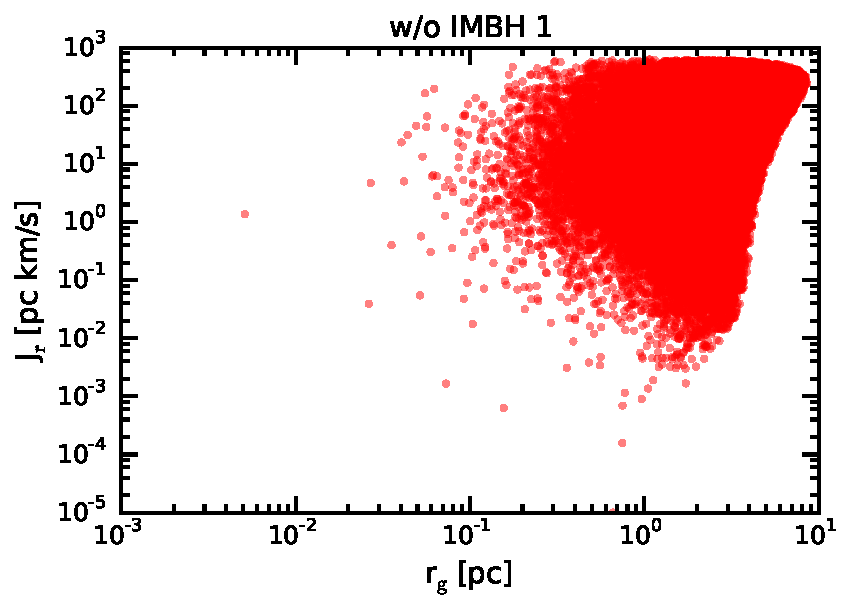
\includegraphics[width=\textwidth]{Plots/r_g_J_r_noIMBH1.pdf}
		\caption{SIM 3}
		\label{fig:r_g_J_r_noIMBH1}
	\end{subfigure}
	\hfill
	\begin{subfigure}{0.475\textwidth}
		\centering
		\includegraphics[width=\textwidth]{Plots/r_g_J_r_noIMBH2.pdf}
		\caption{SIM 4}
		\label{fig:r_g_J_r_noIMBH2}
	\end{subfigure}
	\caption{Radial action over guiding star radius with marked specific stars on loglog scale. All simulations have a similar shaped distributions except for the marked stars which are the specific ones. On the top right corner the shape of \ref{fig:E_J_r_hist_IMBH1} and \ref{fig:E_J_r_hist_IMBH2} is not gently rounded but there are single stars around it. On the lower left there are some extra stars which we identify as the stars with low radial action.}
\end{figure}


\subsection{Discussion \& future perspectives}
do the same distinguishing the mass of the stars\\
redo the work with only observational-like data
\newpage
\section{Conclusion}
In this work we investigated simulated \acp{GC} in orbit space, specifically in action space, to figure out if we can use this method to find signatures of \acp{IMBH}. Given four simulations two of which containing an \ac{IMBH} we first examined the properties in color-magnitude and in phase space. Generating the potentials of the simulations from their density profiles we calculated integrals of motion for all the \ac{GC} stars. Due to the spherically symmetric potential of the \acp{GC} only the energy and the total angular momentum as classical integrals of motion and particularly the radial action as best choice of integral of motions were relevant to us. We found a clear signature of \acp{IMBH} in the distribution of stars in the specific radial action versus specific energy plane. More but less clear signatures were found in a distribution of the radial action versus the guiding star radius and in a distribution of the radial action versus the angular momentum. The robustness of these signatures was tested, using a wrong density as a base of our calculations. Further investigations have to be done, i.e. by changing the Kepler potential of the \ac{IMBH} and comparing the simulations with exact identical initial conditions and as only difference the presence of an \ac{IMBH}. Then we will have to think about how to adapt our method for an application to observational data. 
\newpage 
\section{Acronyms}

\begin{acronym}[SMBH]
	\acro{CMD}{color magnitude diagram}
	\acro{COM}{centre of mass}
	\acro{DF}{distribution function}
	\acro{GC}{globular cluster}
	\acro{v-GC}{Globular clusters}
	\acro{HST}{Hubble Space Telescope}
	\acro{IMBH}{intermediate mass black hole}
	\acro{MW}{Milky Way}
	\acro{SMBH}{super massive black hole}
	\acro{SSP}{single stellar population}
\end{acronym}
\newpage
\bibliography{Literatur}
\addcontentsline{toc}{section}{Bibliography}
\newpage
\hspace{-12pt}{\large\textbf{Acknowledgements}}\\
\\First of all I would like to thank Dr. Glenn van de Ven for welcoming me in his friendly working group and giving me the opportunity to get to know the exciting field of dynamics. I am also thankful for his support by giving useful comments and advices relating my thesis.\\
\\
My gratitude also goes to Prof. Rainer Spurzem for evaluating my thesis.\\
\\
Special thanks to Wilma Trick and Paolo Bianchini for guiding me through my investigations, answering all my questions, helping me coding, giving further suggestion, discussing about results and proof reading my thesis.\\
\\
Furthermore I would like to thank my parents Ivo and Sigrun for giving me the possibility and support to study.  \\
\\
Another big thanks to my boyfriend Alex for supporting me, listening to my problems and helping me with his advice whenever I needed it. \\
\\
Last but not least I would like to thank my office mates, especially Alina and Melanie for helping and pushing each other, and all my other friends.


\newpage
\hspace{-12pt}{\large{\textbf{Erklärung}}}\\
\\
Ich versichere, dass ich diese Arbeit selbstst\"{a}ndig verfasst und keine anderen als die angegebenen Quellen und Hilfsmittel benutzt habe.
\\ \\
Heidelberg, den 03.03.2016,\\
\\
\\
------------------------------------------------------ \\
{\footnotesize Sophia Milanov}


\end{document}